\chapter{Modelowanie fizyczne}
\section{Synteza dźwięku skrzypiec}

Syntezę dźwięku skrzypiec można podzielić na trzy obszary:
\begin{itemize}
	\setlength\itemsep{-3pt}
	\item[--] symulację rozchodzenia się fal w strunie,
	\item[--] symulację interakcji pomiędzy smyczkiem a struną,
	\item[--] symulację przechodzenia fal ze strun do korpusu skrzypiec poprzez mostek.
\end{itemize}
Kompletny schemat blokowy modelu realizującego syntezę dźwięku instrumentu smyczkowego jest pokazany na rysunku \ref{rys:schematblokowy} pochodzącego z \cite{bowed_3}.
\begin{figure}[H]
	\centering
	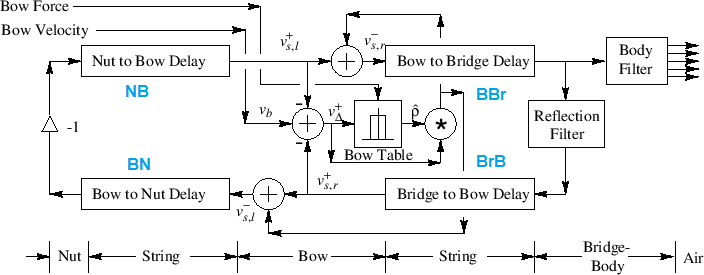
\includegraphics[width=12cm]{grafiki/schematblokowy}
	\captionsetup{justification=centering}
	\caption{Schemat blokowy modelu realizującego syntezę dźwięku.}
	\label{rys:schematblokowy}
\end{figure}

\begin{figure}[H]
	\centering
	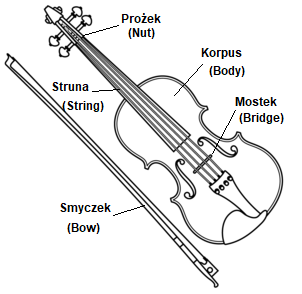
\includegraphics[width=5cm]{grafiki/skrzypce}
	\captionsetup{justification=centering}
	\caption{Elementy skrzypiec istotne dla symulacji.}
	\label{rys:skrzypce}
\end{figure}

W następnych podrodziałach omówione zostaną kolejne obszary symulacji w oparciu o \cite{bowed_smith}. Należy mieć na uwadzę, że ostatecznie synteza tego typu przeprowadzana jest na DSP w czasie rzeczywistym.


\subsection{Rozchodzenie się fal w strunie}
Rozchodzenie się fal w strunie jest symulowane przy wykorzystaniu cyfrowego falowodu (ang. digital waveguide) oraz filtrów, które mają za zadanie odwzorować odbijanie się fal na końcach struny. Fale rozchodzące się w strunie wpływają na prędkość lokalnych odchyleń tej struny. Ta prędkośc wraz z prędkością przesuwania smyczkiem po strunie stanowią podstawę do syntezy dźwięku skrzypiec.

\subsubsection{Linia opóźniająca}
Linia opóźniająca (ang. delay line) to element wprowadzający opóźnienie czasowe pomiędzy próbkami, które otrzymuje na wejściu, a próbkami, które z niego wychodzą. 
\begin{figure}[H]
	\centering
	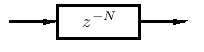
\includegraphics[width=5cm]{grafiki/linia}
	\captionsetup{justification=centering}
	\caption{Linia opóźniająca o długości N.}
	\label{rys:delay_line}
\end{figure}
Na rysunku \ref{rys:delay_line} przedstawiona została linia opóźniająca o długości N próbek. Implementacja tego elementu sprowadza się do tablicy o N elementach oraz wskaźnikach na pierwszy i ostatni element. W celu uzyskania opóźnień czasowych o niecałkowitą liczbę próbek, stosuje się prostą interpolację liniową pomiędzy dwoma sąsiednimi próbkami.
\subsubsection{Cyfrowy falowód}
Cyfrowy falowód jest zdefiniowany jako dwukierunkowa linia opóźniająca. Implementuje się go zatem jako dwie linie opóźniające, w których fale rozchodzą się w przeciwnych kierunkach. Cyfrowy falowód można interpretować jako strunę - dłuższa struna będzie wiązała się z dłuższym falowodem. Oznacza to, że można określić prędkość odchylania się struny w dowolnym punkcie jej długości. Dokonuje się tego poprzez sumowanie, w danym punkcie struny, prędkości fali rozchodzącej się w jednym kierunku oraz predkości fali rozchodzącej się w drugim kierunku.
\subsubsection{Odbicia na końcach struny}
Fale w strunie rozchodzą się w obu kierunkach, aż dotrą do końca struny - mostka, prożka lub palca skrzypka. Elementy te, oznaczone na rysunku \ref{rys:skrzypce}, uniemożliwiają strunie ruch, zatem fale się od nich odbijają. Fala, która dociera do jednego z tych elementów, zostaje częściowo odbita, więc zmienia się jej kierunek rozchodzenia. Odbijanie implementowane jest jako przepisywanie danej próbki z końca jednej linii opóźniającej do początku drugiej w obrębie jednego cyfrowego falowodu. Przy takim odbiciu następuje zmiana znaku próbki.
Dodatkowo, aby uwzględnić straty zachodzące przy odbiciach oraz samym rozchodzeniu się fali, co najmniej jedno odbicie modeluje się za pomocą filtra dolnoprzepustowego o wzmocnieniu mniejszym od 1.


\subsection{Interakcja pomiędzy smyczkiem a struną}
Smyczek przesuwany po strunie, na skutek tarcia pomiędzy jego włosiem a struną, wprawia ją w ruch. Dopóki siła tarcia jest większa niż siła sprężystości struny, to struna odchyla się zgodnie z ruchem smyczka. Jednak w momencie kiedy siła sprężystości będzie odpowiednio duża, struna przestanie podążać za smyczkiem i wykona gwałtowny ruch w kierunku przeciwnym do przesuwania smyczka.  Cykl ten się powtarza przez cały czas trwania pojedynczego przejazdu smyczka po strunie.  \\
Wykres współczynnika tarcia w zależności od różnicy pomiędzy prędkościami struny oraz smyczka pokazano na rysunku \ref{rys:tarcie}. Jako że zmienną kontrolowaną jest prędkość wychylenia struny, wykorzystuje się współczynnik odbicia, którego wykres przedstawiono na rysunku \ref{rys:tarcie}. Przy wartości równej $1$ współczynnika odbicia $\rho$, struna podąża za smyczkiem. Im wartość $\rho$ jest mniejsza, tym większy jest poślizg struny.

\begin{figure}[H]
	\centering
	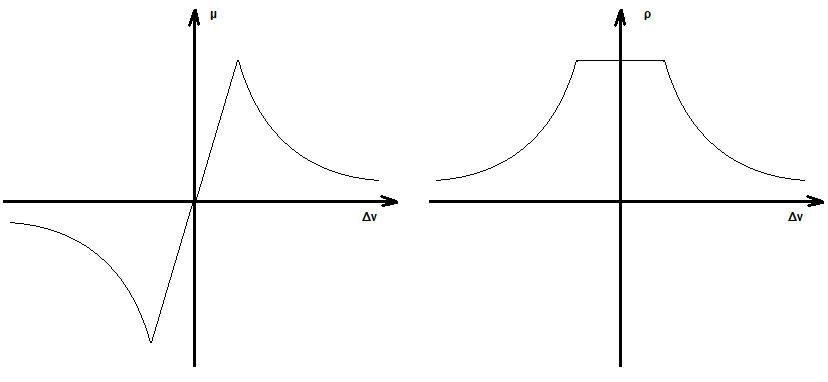
\includegraphics[width=10cm]{grafiki/tarcie2}
	\captionsetup{justification=centering}
	\caption{Współczynnik tarcia $\mu$ w funkcji różnicy prędkości struny i smyczka (po lewej) oraz współczynnik odbicia $\rho$ (po prawej).}
	\label{rys:tarcie}
\end{figure}

Wartości współczynnika odbicia $\rho$ są wyliczane raz i przechowywane w tablicy. Następnie wyznacza się różnicę pomiędzy prędkościami struny oraz smyczka $v_{diff}$:
\begin{equation} \label{equ:wzor1}
v_{diff}[t] = v_b[t] - v_{l}^{+} - v_{r}^{+}
\end{equation}
\begin{tabular}{ l l l l}
	gdzie: & $t$ &  - & obecna chwila czasu, \\
	&	$v_b$ & - &  prędkość smyczka, \\
	&	$v_{l}^{+}$ & - & prędkość struny przychodząca wraz z falą z lewej strony,\\
	&	$v_{r}^{+}$ & - &  prędkość struny przychodząca wraz z falą z prawej strony.\\
\end{tabular} \\ \\
I dalej wyznaczone zostają prędkości struny, które rozejdą się od smyczka odpowiednio w lewą i prawą stronę:
\begin{equation} \label{equ:wzor2}
v_{l}^{-} = v_r^{+} +  \rho(v_{diff}[t])v_{diff}[t]
\end{equation}
\begin{equation} \label{equ:wzor3}
v_{r}^{-} = v_l^{+} +  \rho(v_{diff}[t])v_{diff}[t]
\end{equation}
\begin{tabular}{ l l l l}
	gdzie: & $\rho$ &  - & stablicowana funkcja przedstawiona na rysunku \ref{rys:tarcie}. \\
	
\end{tabular}
\vspace{6pt}

W wyniku pobudzania smyczkiem, struna wpada w charakterystyczny ruch, który jest nazywany ruchem Helmholtza. Jak pokazano w \cite{bowed_2}, próbkowanie prędkości wychyleń struny - będącej w ruchu Helmholtza - w danym punkcie jej długości, daje sygnał zbliżony do przebiegu piłokształtnego. Zgadza się to z wcześniej opisanym zjawiskiem cyklicznego podążania struny wraz ze smyczkiem oraz ślizgania się po nim.

\subsection{Przechodzenie fal ze strun do korpusu skrzypiec} 

Ostatnim etapem jest przenoszenie się fal akustycznych ze strun do korpusu skrzypiec, które zachodzi w mostku. Później korpus drgając wprowadza te fale do powietrza i tak powstaje słyszalny dźwięk. W tym celu bada się funkcję przenoszenia pomiędzy mostkiem a powietrzem. 

W \cite{bowed_smith} do zbadania transmitancji mostek-korpus, zaproponowano metodę, w której sygnałem wyjściowym jest dźwięk w powietrzu, a sygnałem wejściowym jest siła działająca na mostek. Przyjęcie siły jako sygnału na wejściu tego układu wynika z tego, że mostek jest nieruchomym mocowaniem struny. Zatem prędkość mostka jest znikoma. Na mostek unieruchamiający wibrującą strunę działa siła wynikająca z prędkości odchyleń tej struny. W przytoczonej pracy, do pomiaru dźwięku został wykorzystany mikrofon, umieszczony w odległości około jednej stopy od czoła instrumentu, oraz przetwornik piezoelektryczny, przyklejony żywicą epoksydową do mostka, co pokazano na rysunku \ref{rys:pomiary}. Aby uzyskać jak najlepszy stosunek sygnału do szumu sygnału wyjściowego, mikrofon nie może znajdować się zbyt daleko oraz same pomiary powinny być przeprowadzane w komorze bezechowej.

\begin{figure}[H]
	\centering
	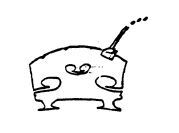
\includegraphics[width=5cm]{grafiki/pomiary}
	\captionsetup{justification=centering}
	\caption{Przetwornik piezoelektryczny przyklejony do mostka skrzypiec.}
	\label{rys:pomiary}
\end{figure}

Spróbowano rozmaitych sposobów pobudzania struny: prostego smyczkowania, techniki glissando, ze strunami owiniętymi tkaniną (próbowano uchwycić szum, syczenie smyczka lekko przesuwanego po strunie w pobliżu mostka), uderzania przetwornika śrubokrętem oraz szarpania strun kostką gitarową w pobliżu mostka. Najlepsze wyniki uzyskano dla tego ostatniego sposobu.

Uzyskane w ten sposób widmo częstotliwościowe poddano odpowiedniej obróbce. Między innymi zmniejszono częstotliwość próbkowania oraz wygładzono przebieg widma. Następnie próbowano dopasować do niego proces autoregresyjny używając różnych metod identyfikacji. Ostatecznie najlepszy wynik uzyskano stosując normę Hankela, a ostateczne dopasowanie charakterystyk pokazano na rysunku \ref{rys:hankel}.

\begin{figure}[H]
	\centering
	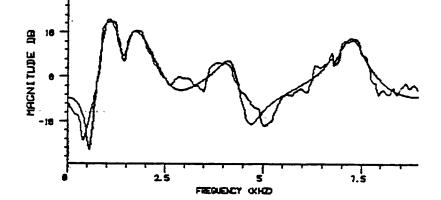
\includegraphics[width=8cm]{grafiki/hankel}
	\captionsetup{justification=centering}
	\caption{Dopasowanie widma amplitudowego procesu AR do pomierzonego.}
	\label{rys:hankel}
\end{figure}

Autorzy \cite{bowed_4} przeprowadzili podobne pomiary, z tym, że strunę pobudzali młotkiem wyposażonym w piezoelektryczny miernik siły, a mikrofon umieścili metr od instrumentu.

W \cite{bowed_2} pomiarów dokonano nieco inaczej. W opisanej tam metodzie, wykorzystany został młotek wyposażony w czujnik siły. Młotkiem tym uderzano w mostek w kierunku prostopadłym do strun. Na mostku z kolei, zamontowany był akcelerometr mierzący przyspieszenie również w kierunku prostopadłym do strun.

Wszystkie te działania zmierzały do zidentyfikowania modelu autoregresyjnego, który odworowuje szczyty rezonansowe pomierzonego widma częstotliwościowego. Model ten jest pobudzany sygnałem uzyskanym z próbkowania prędkości struny. Uzyskane w ten sposób wyjście to dźwięk skrzypiec.
